\documentclass{ximera}

\outcome{Why does $f'(x)$ tell us whether $f(x)$ is increasing or decreasing?}
\outcome{How do we find local maximums and minimums?}
\outcome{What are concavity and inflections points?}
\outcome{When can we find an absolute maximum or minimum on an open interval?}
\outcome{Find the intervals where a function is increasing or decreasing.}
\outcome{Find the intervals where a function is concave up or down.}
\outcome{Find all local maximums and minimums using the 1st and 2nd derivative tests.}
\outcome{Determine when a local extrema is an absolute extrema.}
\outcome{Sketch a graph of $f(x)$ with information from $f'(x)$.}

\title{What derivatives tell us}

\begin{document}

\begin{abstract}
  We gain much information about a differentiable function from the
  sign of its derivative.
\end{abstract}
\maketitle


\section*{The First Derivative Test}

We can use information about the derivative to decide if a critical
point is a local maximum or minimum. Recall that

\begin{itemize}
\item If $f'(x) >0$ on an interval, then $f(x)$ is increasing on that interval.
\item If $f'(x) <0$ on an interval, then $f(x)$ is decreasing on that interval.
\end{itemize}

\begin{question}
True or false: If $f'(x)>0$, then $f(x)$ is positive. 
    \begin{multipleChoice}
      \choice[correct]{False}
      \choice{True}
    \end{multipleChoice}  
\end{question}


So how exactly does the derivative tell us whether there is a maximum,
minimum, or neither at a point? Use the \textit{first derivative test}.

\begin{theorem}[First Derivative Test]
Suppose that $f(x)$ is continuous on an interval, and that $f'(a)=0$
for some value of $a$ in that interval.
\begin{itemize}
\item If $f'(x)>0$ to the left of $a$ and $f'(x)<0$ to the right of
  $a$, then $f(a)$ is a local maximum.
\item If $f'(x)<0$ to the left of $a$ and $f'(x)>0$ to the right of
  $a$, then $f(a)$ is a local minimum.
\item If $f'(x)$ has the same sign to the left and right of $a$,
  then $f(a)$ is not a local extremum.
\end{itemize}
\end{theorem}

\begin{question}
True or false: If $f'(6)=0$ and $f(7)>f(6)$ and $f(5)>f(6)$ then we
must conclude that $x=6$ is a local minimum.
    \begin{multipleChoice}
      \choice[correct]{False}
      \choice{True}
    \end{multipleChoice}  
\end{question}




\section*{Concavity and Inflection Points}

We know that the sign of the derivative tells us whether a function is
increasing or decreasing. Likewise, the sign of the second derivative
$f''(x)$ tells us whether $f'(x)$ is increasing or decreasing. We
summarize this in the table below:
\[
\begin{array}{c|c|c|} %% gives thick lines
 & f'(x)<0 & f'(x) > 0 \\ \hline & & \\[-1.5ex]
f''(x)> 0 & 
\begin{minipage}{2in}
\[
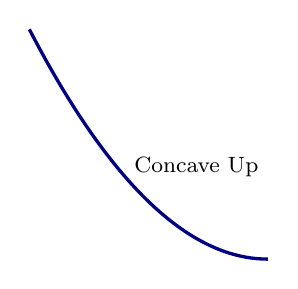
\begin{tikzpicture}
    \colorlet{textColor}{black}
    \colorlet{penColor}{blue!50!black}
	\begin{axis}[
            clip=false,
            height=4.5cm,
            domain=0:1,
            ymax=1,
            ymin=0,
            axis lines=none,
          ]
          \addplot [very thick, penColor, smooth] {(x-1)^2};
          \node at (axis cs:.7,.4) [textColor] {\footnotesize Concave Up};
        \end{axis}
\end{tikzpicture}
\]
\begin{minipage}{2in}\footnotesize
Here $f'(x)<0$ and $f''(x)>0$. This means that $f(x)$ slopes down and
is getting \textit{less steep}. In this case the curve is
\textbf{concave up}.
\end{minipage}
\end{minipage}
&
\begin{minipage}{2in}
\[
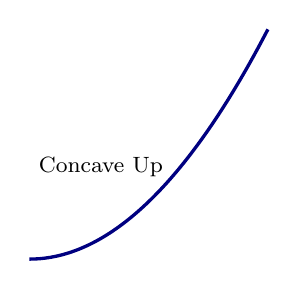
\begin{tikzpicture}
    \colorlet{textColor}{black}
    \colorlet{penColor}{blue!50!black}
	\begin{axis}[
            clip=false,
            domain=0:1,
            ymax=1,
            height=4.5cm,
            ymin=0,
            axis lines=none,
          ]
          \addplot [very thick, penColor, smooth] {x^2};
          \node at (axis cs:.3,.4) [textColor] {\footnotesize Concave Up};
        \end{axis}
\end{tikzpicture}
\]
\begin{minipage}{2in}\footnotesize
Here $f'(x)>0$ and $f''(x)>0$. This means that $f(x)$ slopes up and is
getting \textit{steeper}. In this case the curve is \textbf{concave
  up}.
\end{minipage}
\end{minipage}
\\[-2ex]
& & 
\\\hline 
& & \\[-1.5ex]
f''(x)<0 &
\begin{minipage}{2in}
\[
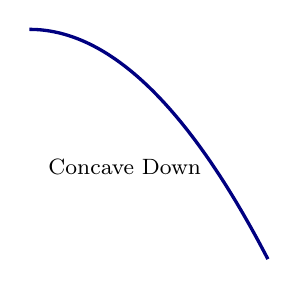
\begin{tikzpicture}
  \colorlet{textColor}{black}
  \colorlet{penColor}{blue!50!black}
	\begin{axis}[
            clip=false,
            height=4.5cm,
            domain=0:1,
            ymax=1,
            ymin=0,
            axis lines=none,
          ]
          \addplot [very thick, penColor, smooth] {-x^2+1};
          \node at (axis cs:.4,.4) [textColor] {\footnotesize Concave Down};
        \end{axis}
\end{tikzpicture}
\]
\begin{minipage}{2in}\footnotesize
Here $f'(x)<0$ and $f''(x)<0$. This means
that $f(x)$ slopes down and is getting \textit{steeper}. In this case the curve is \textbf{concave down}.
\end{minipage}
\end{minipage}
&
\begin{minipage}{2in}
\[
  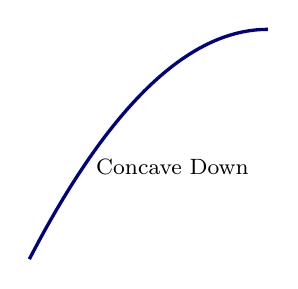
\begin{tikzpicture}
    \colorlet{textColor}{black}
    \colorlet{penColor}{blue!50!black}
	\begin{axis}[
            clip=false,
            height=4.5cm,
            domain=0:1,
            ymax=1,
            ymin=0,
            axis lines=none,
          ]
          \addplot [very thick, penColor, smooth] {-(x-1)^2+1};
          \node at (axis cs:.6,.4) [textColor] {\footnotesize Concave Down};
        \end{axis}
\end{tikzpicture}
\]
\begin{minipage}{2in}\footnotesize
Here $f'(x)>0$ and $f''(x)<0$. This means
that $f(x)$ slopes up and is getting less \textit{steep}. In this case the curve is \textbf{concave down}.
\end{minipage}
\end{minipage}
\\[-2ex]
& & 
\\\hline 
\end{array}
\]

If we are trying to understand the shape of the graph of a function,
knowing where it is concave up and concave down helps us to get a more
accurate picture. It is worth summarizing what we have seen already in
to a single theorem.

\begin{theorem}[Test for Concavity]
Suppose that $f''(x)$ exists on an interval.
\begin{enumerate}
\item If $f''(x)>0$ on an interval, then $f(x)$ is concave up on that interval.
\item If $f''(x)<0$ on an interval, then $f(x)$ is concave down on that interval.
\end{enumerate}
\end{theorem}


Of particular interest are points at which the concavity changes from
up to down or down to up. 

\begin{definition}
If $f(x)$ is continuous and its concavity changes either from up to
down or down to up at $x=a$, then $f(x)$ has an \textbf{inflection
  point} at $x=a$.
\end{definition}


\begin{question}
True or false: If $f''(a) = 0$, then $x=a$ is an inflection point.
    \begin{multipleChoice}
      \choice[correct]{False}
      \choice{True}
    \end{multipleChoice}  
\end{question}



It is instructive to see some examples and nonexamples of inflection
points.
\[
\begin{array}{cccc}
\begin{tikzpicture}
  \colorlet{textColor}{black}
  \colorlet{penColor}{blue!50!black}
	\begin{axis}[
            domain=0:2,
            ymax=2,
            height=4.5cm,
            ymin=0,
            axis lines=none,
          ]
          \addplot [very thick, penColor, smooth, domain=(0:1)] {(x-1)^2+1};
          \addplot [very thick, penColor, smooth, domain=(1:2)] {-(x-1)^2+1};
          \addplot[color=penColor,fill=penColor,only marks,mark=*] coordinates{(1,1)};
        \end{axis}
\end{tikzpicture}

&

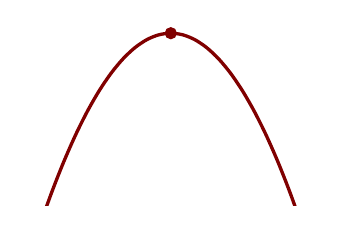
\begin{tikzpicture}
  \colorlet{textColor}{black}
  \colorlet{penColor2}{red!50!black}
	\begin{axis}[
            height=4.5cm,
            domain=0:2,
            ymax=1,
            ymin=0,
            axis lines=none,
          ]
          \addplot [very thick, penColor2, smooth] {-(x-1)^2+.75};
          \addplot[color=penColor2,fill=penColor2,only marks,mark=*] coordinates{(1,.75)};
        \end{axis}
\end{tikzpicture} 

&

\begin{tikzpicture}
  \colorlet{textColor}{black}
  \colorlet{penColor}{blue!50!black}
	\begin{axis}[
            height=4.5cm,
            domain=0:2,
            ymax=2,
            ymin=0,
            samples=100,
            axis lines=none,
          ]
          \addplot [very thick, penColor, smooth,domain=(1:2)] {sqrt(x-1)+1};
          \addplot [very thick, penColor, smooth,domain=(0:1)] {-sqrt(abs(1-x))+1};
          \addplot[color=penColor,fill=penColor,only marks,mark=*] coordinates{(1,1)};
        \end{axis}
\end{tikzpicture}

&

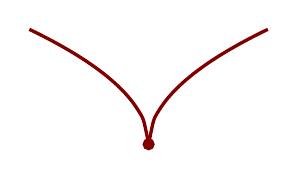
\begin{tikzpicture}
    \colorlet{textColor}{black}
    \colorlet{penColor2}{red!50!black}
	\begin{axis}[
            height=4.5cm,
            domain=0:2,
            ymax=2,
            ymin=0,
            axis lines=none,
          ]
          \addplot [very thick, penColor2, smooth,domain=(1:2)] {sqrt(x-1)+.5};
          \addplot [very thick, penColor2, smooth,domain=(0:1)] {sqrt(abs(1-x))+.5};
          \addplot[color=penColor2,fill=penColor2,only marks,mark=*] coordinates{(1,.5)};
        \end{axis}
\end{tikzpicture} \\

\begin{minipage}{2in}\footnotesize
This is an inflection point. The concavity changes from concave up to
concave down.
\end{minipage}

& 

\begin{minipage}{2in}\footnotesize
This is \textbf{not} an inflection point. The curve is concave down on either side of the point.
\end{minipage}

& 

\begin{minipage}{2in}\footnotesize
This is an inflection point. The concavity changes from concave up to concave down.
\end{minipage}

&

\begin{minipage}{2in}\footnotesize
This is \textbf{not} an inflection point. The curve is concave down on either side of the point.
\end{minipage}

\end{array}
\]

We identify inflection points by first finding where $f''(x)$ is zero
or undefined and then checking to see whether $f''(x)$ does in fact go
from positive to negative or negative to positive at these points.

\begin{warning}
Even if $f''(a) = 0$, the point determined by $x=a$ might \textbf{not}
be an inflection point.
\end{warning}


\begin{question}
Write down at least \textbf{five} questions for this lecture. After
you have your questions, label them as ``Level 1,'' ``Level 2,'' or ``Level 3'' where:
\begin{description}
\item[Level 1] Means you know the answer, or know exactly how to do this problem.
\item[Level 2] Means you think you know how to do the problem, or will soon learn how to do the problem.
\item[Level 3] Means you have no idea how to do the problem. 
\end{description}
  \begin{freeResponse}
  \end{freeResponse}
\end{question}

\end{document}
